 
%%%%%%%%%%%%%%%%%%%%%%%%%%%%%%%%%%%%%%%%%%%%%%%%%%%%%%%%%%%%%%%%%%%%%%%%%%
% Artifacts candidates figure                                            %
%%%%%%%%%%%%%%%%%%%%%%%%%%%%%%%%%%%%%%%%%%%%%%%%%%%%%%%%%%%%%%%%%%%%%%%%%%

\begin{figure}[!b]
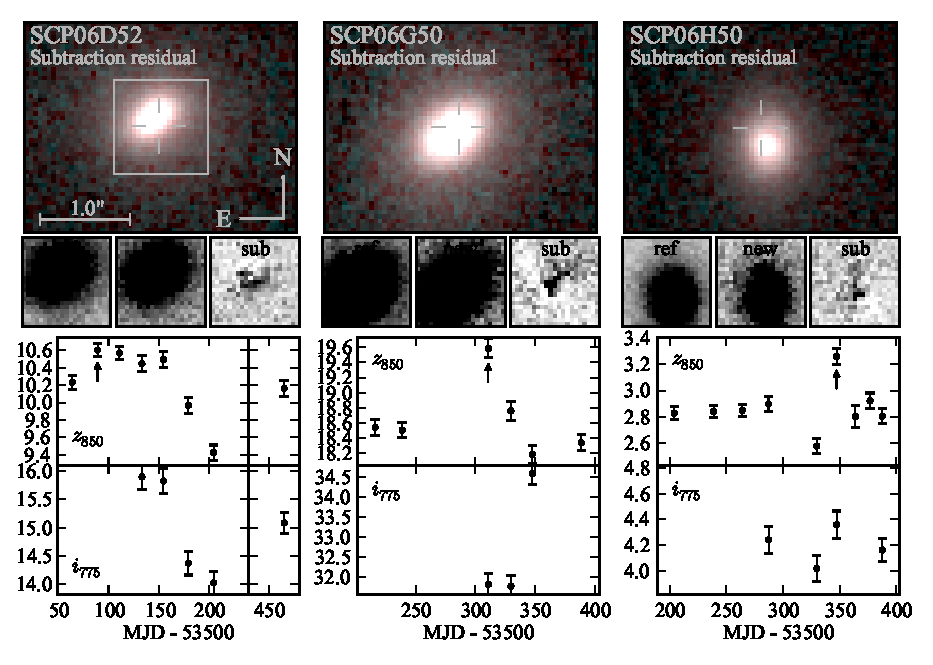
\includegraphics[width=\textwidth]{figures/cands/artifacts1.eps}
\caption[Images and light curves of candidates classified as artifacts]
        {Images and light curves of the candidates classified as image
         artifacts (cosmic ray hits and/or subtraction residuals). For
         each candidate, the \emph{top panel} shows the two-color
         stacked image ($i_{775}$ and $z_{850}$) of the host galaxy,
         with the position of the transient indicated.  The \emph{three
         smaller panels} below the stacked image show the reference,
         new, and subtracted images for the discovery visit. The \emph{bottom
         panel} shows the light curve at the transient position (including
         host galaxy light) in the $z_{850}$ ({\it top}) and $i_{775}$
         ({\it bottom}) bands. The y axes have units of counts per
         second in a $3$~pixel radius aperture. The effective
         zeropoints are 23.94 and 25.02 for $z_{850}$ and $i_{775}$,
         respectively. The discovery visit is indicated with an arrow
         in the $z_{850}$ plot. [\emph{Continued on next three pages.}]
         \label{fig:artifacts}}
\end{figure}

\begin{figure}[p]
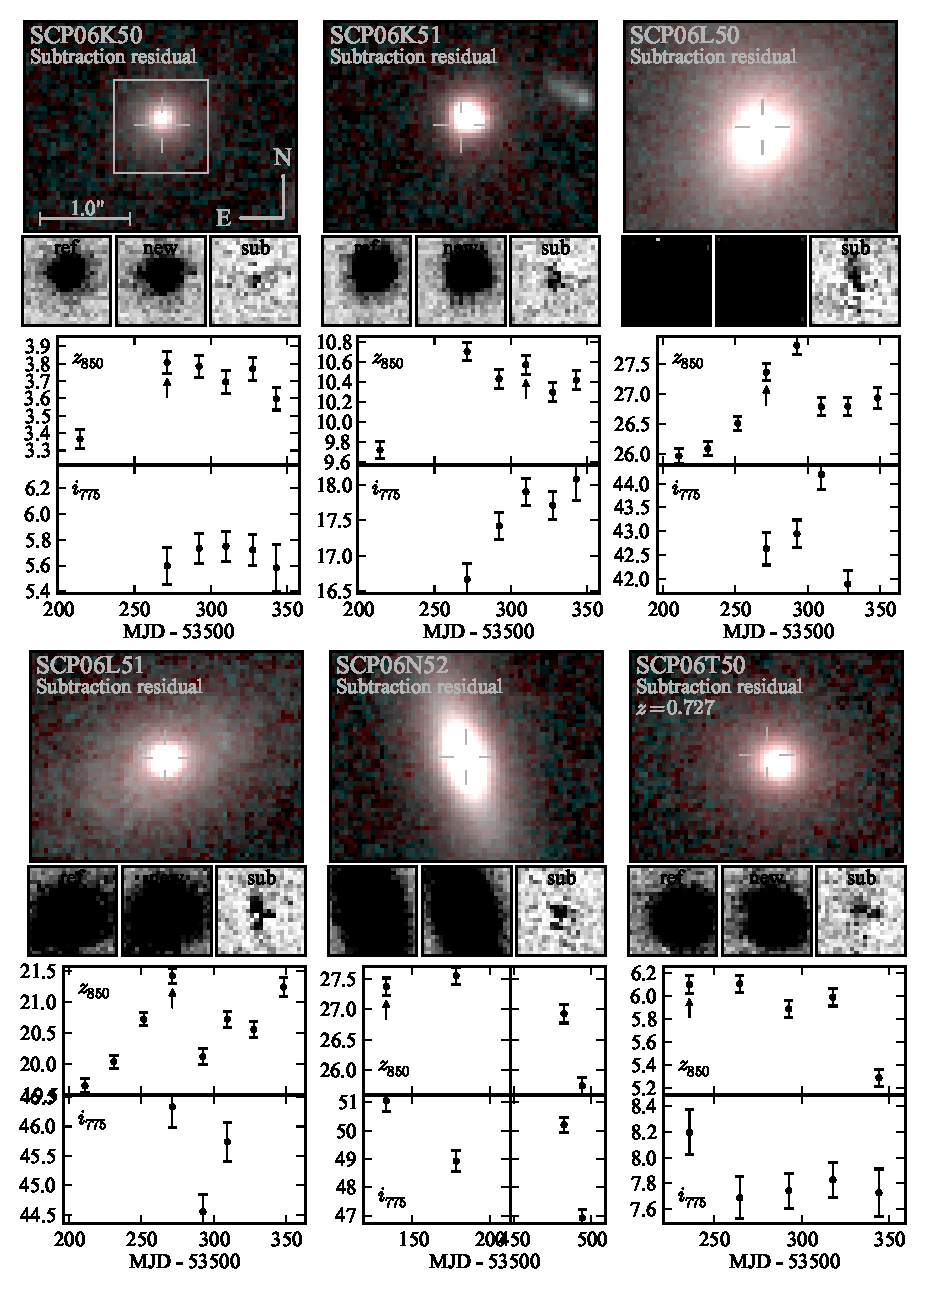
\includegraphics[width=\textwidth]{figures/cands/artifacts2.eps}
\end{figure}

\begin{figure}[p]
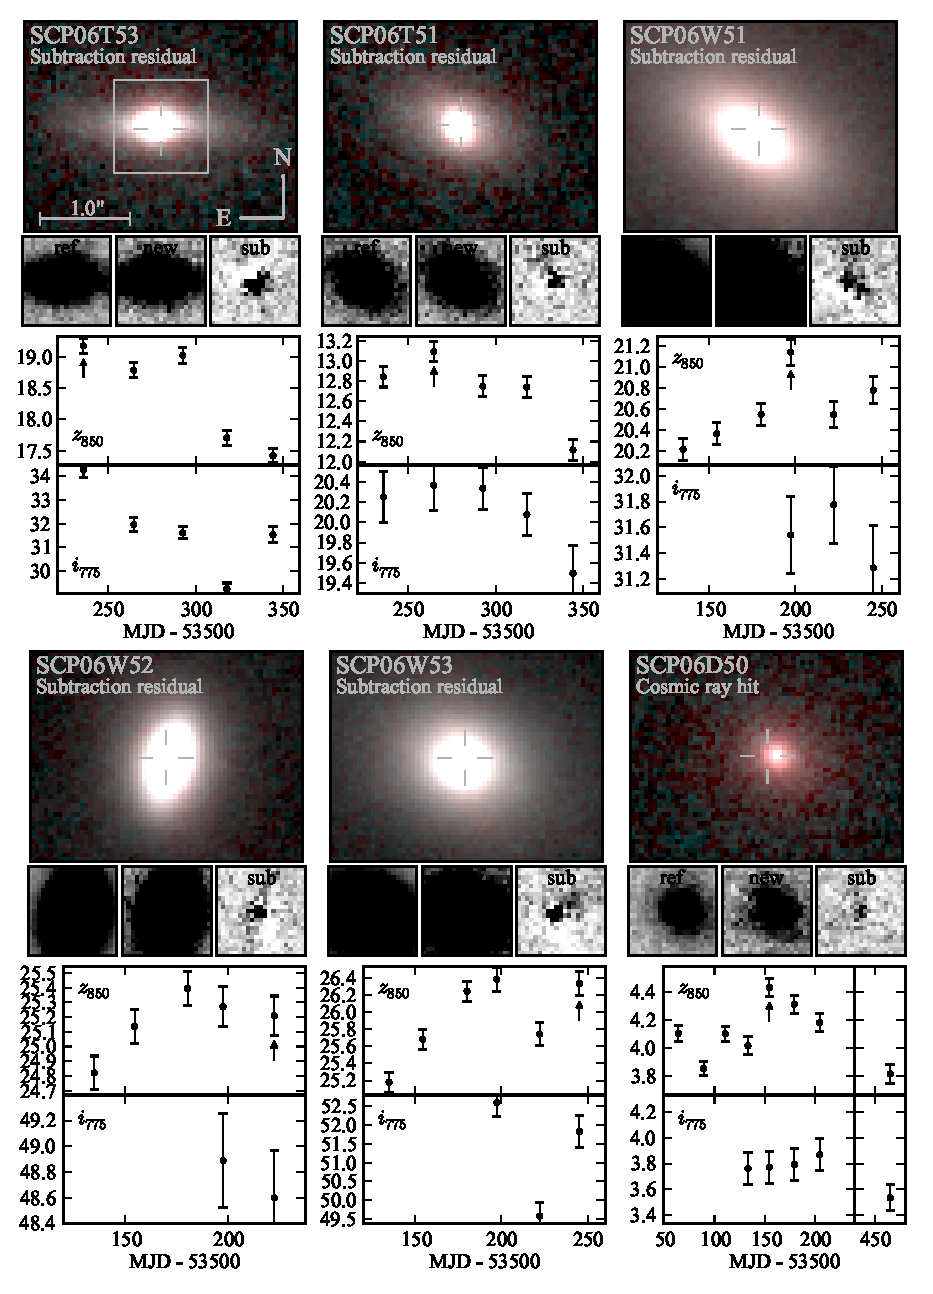
\includegraphics[width=\textwidth]{figures/cands/artifacts3.eps}
\end{figure}

\begin{figure}[t]
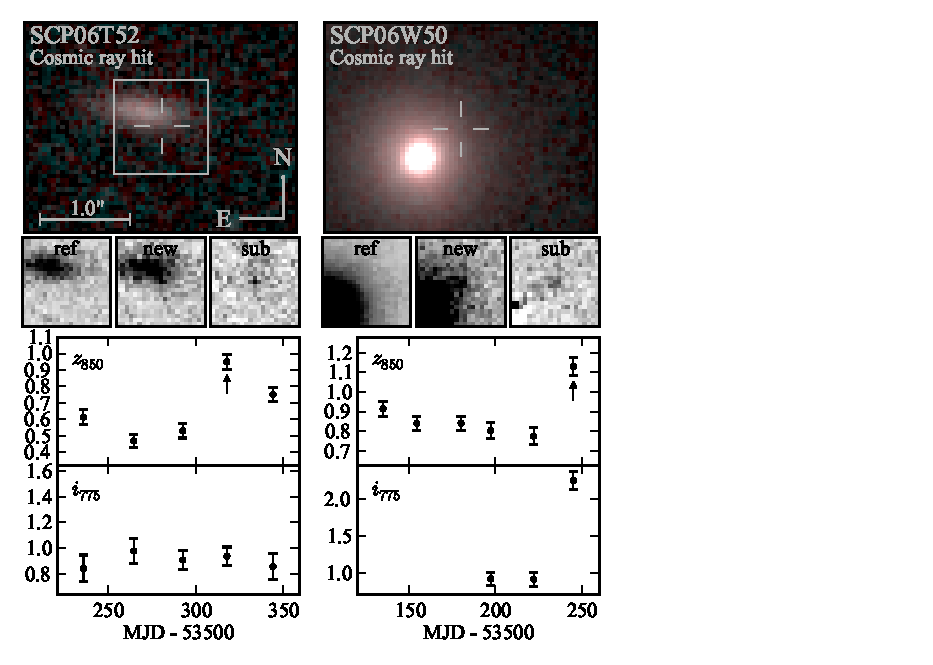
\includegraphics[width=\textwidth]{figures/cands/artifacts4.eps}
\end{figure}

Although the automated selections were designed to eliminate image
artifacts such as subtraction residuals and cosmic rays, they were
made to be somewhat tolerant so that real SNe were not eliminated. The
result is that some artifacts slip through. Candidates located close
to the cores of relatively bright galaxies that show adjoining
negative and positive areas in subtractions are likely to be caused by
mis-alignment between the reference and search image. For such
candidates, we inspected the full light curve for consistency with the
general shape of a SN~Ia light curve. For fourteen of these, the
light curve is completely inconsistent with that of a SN~Ia. Their
light curves have either multiple peaks, long flat portions followed
by one or two lower points, and/or $i_{775}$ data that shows no
change. We classify these fourteen candidates as subtraction residuals
with negligible classification uncertainty (very unlikely that any are
SNe~Ia). These candidates are shown in Figure~\ref{fig:artifacts}.
%Additionally, the peak-to-peak change in $z_{850}$ flux is
%typically too small to be compatible with a SN~Ia, given that the
%galaxies are generally too bright and too blue to be at high
%redshift. For example, seven candidates are on galaxies of $z_{850} <
%20$), yet show peak-to-peak magnitude changes of only $z_{850} \gtrsim
%23.3$, too dim for a SN~Ia at such redshifts.

Candidates where one or two of the four $z_{850}$ exposures was
clearly affected by a cosmic ray or hot pixel may be false
detections. These can pass the automated cosmic ray rejection when
they occur on a galaxy.  For two such candidates, we used the lack of
any change in the $i_{775}$ light curve to rule out a SN~Ia: fitting
SN templates with a range of redshifts and extinctions resulted in
observed $i_{775}$ fluxes too low by $4\sigma$ or more, given the
$z_{850}$ increase. One other candidate, SCP06W50, is less certain. It
was discovered in the last visit to the cluster, making it difficult
to constrain a template light curve. There is clearly a hot pixel or
cosmic ray in one $z_{850}$ exposure, but there appears to be some
excess flux in the other three exposures as well. Also, there is a
point-source like detection in $i_{775}$, but offset $\sim$1.2~pixels
from the $z_{850}$ detection. While the $i_{775}$ detection may also
be a cosmic ray, it is possible that this candidate is a SN caught
very early. The elliptical ``host'' galaxy was not observed
spectroscopically, but we estimate its redshift to be $0.60 < z < 0.85$
based on the color of $i_{775} - z_{850} = 0.55$ and stellar
population models of \citet[][hereafter BC03]{bruzual03a}.

Of the 17 total candidates classified as image artifacts, SCP06W50 is the
only one with significant uncertainty. However, this uncertainty does
not affect the cluster SN~Ia rate as the host galaxy is clearly in the
cluster foreground.
